% =========================================================================

\chapter{Introduction}

Memory usage is one of the most fundamental principles in computing, both
historical and modern. Every program needs some storage - if only for storing
itself somewhere. Modern computing environments contain lot of memory layers on
different levels. There is persistent storage (harddisks, SDD drives), operating
memory, several levels of CPU caches and registers. Usage of all of these is
usually abstracted by the operating systems, which provide the safe access to
these resources to the userspace applications. Technical advancement in recent
age caused the prices of hardware providing storage to go down, so in most causes
totally effective usage of these resources is not an outstanding issue when
programming. The storage is usually relatively cheap to the price of work an
expert programmer has to do to exploit the resources effectively. However,
sometimes the effectiveness matters, especially in some specific areas. Some
major projects are suffering by the performace hit introduced by the currently
used allocators, and invested time and resources to the creation of new
allocators which will solve their problem. The example of this is Google writing
TCmalloc for improved performance of multithreaded applications, or OpenLDAP
project considering changing the allocator from ptmalloc2 (the glibc default) to
improve the performace \cite{openldap-pres}. This thesis attempts to provide a
tool for an analysis of various memory allocators' characteristics under
different usage scenarios.

\section{Motivation}

Dynamically allocated memory is a memory allocated not during compile time, but
on runtime. The reasons vary---the amount of memory needed can be computed from
variables known at runtime, or the memory is needed just for the limited amount
of time and so it would be ineffective to hold it for the whole runtime. The
concept is almost as old as modern computing itself. It seems to be present and
used since the 1960s \cite{DSAsurvey}. In C language, which is still mostly used
in system programming in Linux world, this concept is present in the omnipresent
malloc/free interface \cite{glibc-man-malloc}. Of course, this interface is
present and widely used for a very long time, so the concepts are already
researched thoroughly. There are some very efficient allocation algorithms in
currently used implementations of malloc. There seems to be little space for some
radical improvements.

However, the effectiveness of a memory allocator is also largely influenced by
the usage pattern of it. Over time, the most used memory allocator
implementations converged towards an implementation which has at least an
acceptable behavior for most of the usage cases. This means that for most cases,
a program has a good probability to perform well with the allocator, but it could
do better with another. Most widely used allocators often provide a way for fine
tuning them for the particular environment \cite{glibc-man-malloc}, but often the
results are not as good as they could be if the allocator was made specifically
for the specific usage pattern, sacrificing performance of another cases.

The good example of this case is the program concurrence. For handling multiple
threads allocating memory concurrently, the allocator has to have some mechanism
avoiding conflicts, like locks. An universal allocator does not know whether
program using it is concurrent or not. A lot of programs use threads, so it needs
to have some overhead for them. This overhead is completely unnecessary for
single-threaded programs, and better performance would probably be achieved if an
allocator without the multi-threaded overhead was used. Such an allocator of
course could not be used as system-wide, universal one. All of this is of course
even more complicated in reality.

The environment also changes in time. The appearance of multi-core CPUs brought
some specific problems with cache usage. It is better to allocate memory in a way
that is cache friendly, that means to arrange memory which is used closely in
time also close spatially, and to avoid writing into memory which is shared among
the CPU caches. When CPUs invalidate each other's caches a lot, the advantage of
having it is lost. Such problems can be avoided with proper memory management.

The advantage of using tuned or alternative memory allocator is often not great
enough to justify additional work. Stock allocators are quite effective in most
cases. But there are cases in which the gain can be quite high. High enough so we
can see a major software gigant creating it's own malloc implementation to solve
their problems with existing implementation \cite{tcmalloc}. Another cases can be
seen in some object-oriented libraries, which implement additional layer of
memory management. The reason is that creating objects does quite a large number
of small allocations, which is not effective enough. So these libraries keep a
pool of preallocated objects on which they do some amount of memory allocation of
their own \cite{glib-memalloc}.

This thesis aims to help with analysing performance of various memory allocator
implementations (and their tunings) by providing a tool which can measure
different performance aspects under various conditions. At the moment, such an
analysis seems to be usually done by micro benchmarks crafted for the actual need
without systematic approach, at least in the open-source software world.

\section{Goals}

The goal of this thesis is to provide a tool for analysing memory allocator
performance. Allocator performance is a vague term - different metrics can be
claimed as important in different situations. The tool should be able to measure
all of the most common ones. These will have to be identified. Also, there are
many factors which influence these metrics. The tool shall allow the user to
specify these factors to make the measurement relevant for the particular
situation.

After the identifying these factors and metrics, the tool will be implemented and
test analysis will be performed on various memory allocation implementations.
This term project does not contain the implementation of this tool, that will be
done in the thesis. Just the high-level design decisions will be made based on
the identified metrics and factors.

\chapter{Dynamic memory allocators}
\label{dsa}

This chapter discusses the principles of dynamic memory allocation system used in
modern GNU/Linux systems. Because {\em performance} is very unclear term when
used in context of allocators, various metrics are analysed as performance ones,
and factors which influence these metrics are discovered.

\section{Dynamic memory allocation}

Dynamic memory allocation is an ubiquitous concept in current programming world.
It originated in the very dawn of modern computing, in 1960s, and was driven by
the need of using the memory resources as effectivelly as possible. Dynamic
memory allocation occurs at run-time, where a running program asks the operating
system (or more generally, the memory resource manager) for more memory for its
needs. This is a direct opposite of compile-time {\em static} allocation. There
are more reasons for postponing allocation to runtime. The most significant ones
are:
\begin{enumerate}
\item The exact amount of needed memory is simply not known during compile-time.
This is the common case: the program simply does not know how long e.g. the input
will be.
\item The program needs various amounts of memory in time. Such a memory could
possibly be allocated at compile-time if the size is known: simply the maximum of
the memory consumption would be allocated. That would mean wasting the memory,
because the program would have allocated a lot of memory even when it uses all of
it for only a small portion of runtime.
\end{enumerate}

Over time, the specifics of the memory usage by programs changed. Historically,
the memory of the computers was very small and expensive, so the need was to
place the data in it as effectively as possible. Today, the needs are different.
It is still a good habit to use the memory effectively, but it is no more that
crucial, because the price of the memory dropped and the capacity rised
dramatically. But the advancement also caused several new problems to emerge.
Modern computers generally have enough of operating memory: the problem is, that
the memory access is very slow compared to the speed of modern CPUs. This is
solved by the fast memory layers in CPU: caches. But fast memory is more
expensive, so the cache sizes are very small when compared to the main operation
memory size. If a program does not use the cache well, it's performance can be
drastically slower than the performance of one that does \cite{drepper-memory}.
The way how the dynamic memory allocator works can affect also the cache
friendliness of the programs---by well placing the memory which has a good
probability of being used together. Similar to this, a bad memory allocator can
also introduce a performance hit if it places the memory badly.

\subsection{DSA specification}

In the scope of this thesis, the term "dynamic memory allocator" means the usual
malloc/free interface as it is known from the C programming language. The
programs use the allocator for obtaining and returning arbitrary amount of
storage space for its own use. These allocations and allocations can occur at any
time and in any order. Allocated memory can be directly addressed by the program
- the access to the storage is done outside of the allocator scope. The allocator
is also completely unaware about what is stored in the allocated memory. This
means that the allocator cannot do any internal management on already allocated
blocks of memory, e.g. moving the allocated blocks so that they are stored
compactly, or possibly compressing them. If such operations were done by the
allocator, the program references to such memory blocks would be rendered
invalid, and such an effect is of course indesirable.

The direct access also means that the allocated memory chunk needs to be
continuous, as opposed to e.g. filesystem storage management. The program cannot
recognize the hole in the storage without the allocator's assistance - so the
hole simply can not exist. {\em Continuous} means continuous in the program's
address space here. It can be assembled from the several pages at the level of
virtual memory in kernel of course---this is totally transparent to the program,
including the allocator itself.

\subsection{DSA concepts}

The allocator operates on some amount of memory, which is usually (but not
necessarilly) continous. Some part of this memory is used for the memory
allocator data - these will be called "metadata" later in this thesis. The rest
of this memory is used for provisioning to a program, and is usually divided into
some number of blocks of various size. When a program makes a request for some
amount of memory, the allocator finds or creates some free block of sufficient
size, marks it as used and gives it's address to the program. If no large enough
block is found, additional memory can be obtained from the operating system using
appropriate system calls, such as {\em mmap} and {\em brk} \cite{sbrk-manpage,
mmap-manpage}. When a memory is freed by the program, the block is marked as
free. Free blocks may be used to satisfy subsequent memory request, or it may be
returned to the operating system. The goal of an allocator is to minimize the
unallocated memory amount, while minimizing also the time cost of this effort.

The allocator can satisfy a small block request by dividing a larger block to
several smaller ones and one of these will be then used for satisfying the
request. Similar to this, when some memory is freed and that memory is adjacent
to some already free block, the allocator can choose to coalesce them to one
larger block. Allocators usually do not coalesce all the blocks they could, but
try to keep a free blocks of various size. The reason for this is simple.
Coalescing everything results in lots of unnecessary coalescing and then
splitting again to satisfy smaller requests, leading to worse performance.

There are few notable constraints which makes the allocator's goal harder. The
allocator cannot control the number, order and the memory size of
allocations---these are determined by a program using the allocator. The
allocator also satisfies one allocation at a time (with the exception of possible
concurrency, which does not affect this problem), without the knowledge about the
future allocation requests. The memory must be provided immediatelly, and once
the allocator selects the memory place for it, it cannot be modified when
additional requests come and better decision could be made, until the program
frees that memory. It can be proven that it is not possible to create a dynamic
memory allocator which will not waste memory by bad decision about chunk
placement \cite{DSAsurvey}.

Two main concepts exist in dynamic memory allocation. The first one uses the heap
exclusively, and a {\tt brk} system call to expand and shrink it. The second one
relies on the {\tt mmap} system call, and uses the anonymous memory outside the
heap. Some allocators are using exclusively one of these concepts, while some
others use the combination of both. The GNU/Linux family of operating systems
usually comes with the GNU C library (usually abbreviated as {\em glibc}). This
library uses a variant of Doug Lea's dlmalloc called ptmalloc2. The improvements
are mostly the for better performance in multi-threaded applications (the "pt"
prefix comes from the term {\em pthreads}, a commonly used abreviation for the
POSIX Threads standard). This allocator uses a combination of the two
concepts---it uses heap for smaller requests and anonymous memory for the larger
ones. Aside from this widespread memory allocator, there are several more
alternative memory allocators used on Linux, usually claiming better performance
in various aspects. The two more popular are Hoard and TCmalloc. Hoard, developed
at the University of Massachusets in Amherst, is a thread oriented memory
allocator using {\tt mmap} exclusively to construct an internal architecture of
per-thread heaps \cite{allocators:hoard}. The second one is also a thread
oriented allocator, called Thread Caching malloc---TCmalloc. TCmalloc uses {\tt
mmap} exclusively and has quite sophisticated system of allocation based on
different allocation strategies based on the request size. It also provides a
thread local cache for quick allocation of small requests to avoid locking
\cite{tcmalloc}. TCmalloc is developed by Google, Inc. Few more experimental
alternative memory allocators do exist, but these do not seem to be used much.

\section{Interesting performance metrics of memory allocators}
\label{metrics}

There is no clear performance metric for memory allocators. There are different
metrics describing the characteristics of an allocator, and their importance and
relevance as a performance metric depends on the characteristics of a program
using this allocator. For example, a time per allocation certainly matters in a
program doing millions of allocations, while it is not much interesting in a
program with only few allocations. This section lists various metrics which can
under some circumstances be considered as relevant performance metrics, along
with these circumstances.

There are two types of performance metrics: time and memory usage. Time metrics
affect the program execution speed in some way. Two time-affecting metrics were
identified: allocation speed, which directly affects the program speed, and
locality, which affects the program speed indirectly by making the program more
or less friendly to CPU cache systems. Memory related metrics are also two:
fragmentation and memory overhead. Memory overhead increases memory usage by
using some memory for the allocator data. Fragmentation means the efficiency of
using disposable memory for provisioning to a program.

\subsection{Memory overhead}
\label{metrics:overhead}

Every memory allocator needs some memory for it's own use. At the very least, it
needs to store the sizes of the memory blocks provided to program, so they can be
marked as unused when freed. There are two possible types of memory overhead: per
allocator, and per allocation. Overhead per allocator means a memory consumption
by {\em global} data structures used by the allocator. This memory will be used
even when no memory is allocated by the program. Some allocators need some
metadata memory for each allocation made by the program. This is per allocation
overhead. Information about the block or about adjacent blocks can be stored in a
{\em header} somewhere, usually at the beginning of the block, just before the
actual block of memory provided to the program. The per allocator overhead size
is not that important, if it is not extremely large - it's only allocated once
and usually does not change much. Per allocation overhead size can be important
under certain conditions. One of the cases when per-allocation overhead is
interesting metric is obviously when program does a large amount of very small
allocations. For example, when per-allocation metadata needs 16 bytes and the
program does a lot of 16 bytes allocations, the amount of memory needed for such
program is twice as high as the amount actually used by it.

There are more reasons why the allocator can create some overhead memory: in
addition to the memory actually used by allocator metadata some memory does not
necessarily need to be used at all. The free unused memory block can be created
when some architecture dependent decisions are made, for example considering
alignment. A figure \ref{fig:overhead} shows the different types of memory
overhead. Memory overhead is sometimes considered to be a type of fragmentation.
Fragmentation is discussed in more details in \ref{metrics:fragmentation}.

\begin{figure}[h]
\begin{center}
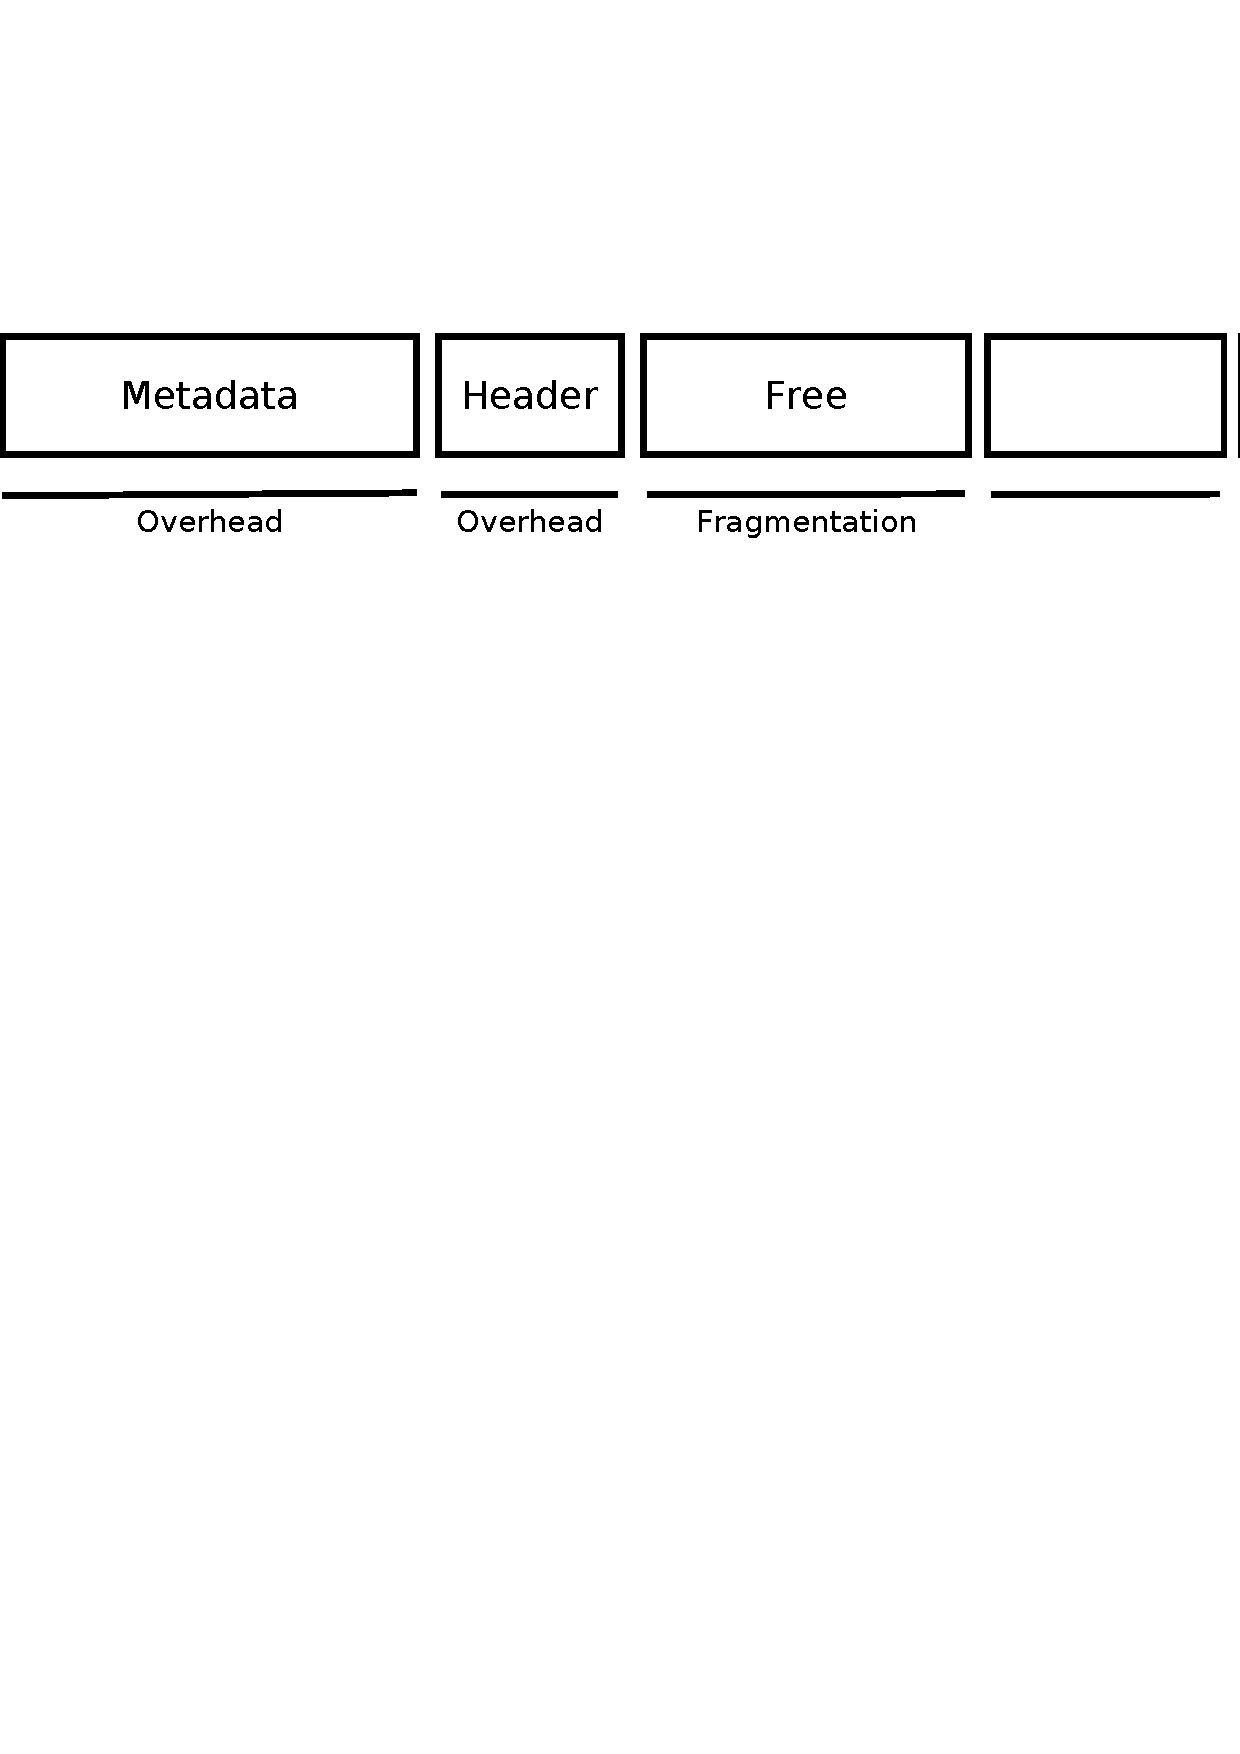
\includegraphics[width=1.0\textwidth,keepaspectratio]{fig/frags}
\end{center}
\caption{The difference between overhead and fragmentation}
\label{fig:overhead}
\end{figure}

\subsection{Allocation speed}

Allocation speed is simply the amount of time spent processing the allocation or
deallocation request. In usual use cases, the allocation speed is not very
important, because allocator requests usually make only a minor portion of
program statements. In such cases, time taken by memory allocation requests is
negligible in the total time the program takes to execute (if the time taken by
the allocator is not extreme, of course), so the performance impact on the
program is low. However, this is not always the case. In some environments where
a large number of allocations and deallocations occurs, the program performance
can rapidly increase and decrease in accordance to the allocator performance. An
example of such environment is the interpreter of some object-oriented scripting
language, such as Python or Ruby. When these interpreters are processing some
scripts, large hierarchies of objects can be created or destroyed (for example
when entering or leaving a function), which results in a large chain of small
allocations or deallocations. Low performance allocator can rapidly decrease
performance of execution of such a program.

\subsection{Locality and spatial layout}

Locality is a metric which can dramatically affect performance of a program.
Current computers have several layers of operating memory - in addition to
"normal" operating memory, current CPUs have several levels of cache memory. For
example, Intel i7 family of CPUs have three levels of cache, and this number is
very common for current CPUs. Usually, the closer the cache level is to the CPU
itself, the faster are the operations with data in it. Reading data from L1 cache
can be 80 times faster than reading same data from the main memory. L2 cache is
cca 17 times faster \cite{drepper-memory}. Smart memory allocator can arrange
data in a way that is friendly to this memory structure: if data, which are often
used together are also placed near themselves in memory, then it is likely that
both can be present in the fastest cache, and thus all the work can be done on
the fast cache level without the need of multiple main memory accesses.
Similarly, poor allocator can place data which are used together in different
memory areas, which then basically eradicates the advantage of having a cache
because of cache trashing.

Allocators can improve their locality metric either by taking advantage of some
common program patterns, or by taking hints from the program it serves. One quite
common pattern is a temporal one. Data which are allocated close in time are
quite likely to be used close in time. So if an allocator places temporally close
allocations also spatially close, it has a good chance of being cache-friendly,
improving the program's performance. Second method is taking hints from the
program itself---the programmer usually knows which data will be used together.

Second issue concerning memory layout is the allocator induced false sharing.
False sharing is a usage pattern where two threads use their objects exclusively,
but theses two objects share a cache line. When one thread modifies its object,
second one will have to read its object from memory again, despite the object was
not modified and it could be safely read. The reason for this is that when the
first CPU wrote its data, whole cache line was rendered as invalid for the other
CPUs. If the allocator places the memory chunks allocated by different threads
close to each other, it can lead to lower program performance because of the
false sharing caused by this.

\subsection{Fragmentation}
\label{metrics:fragmentation}

Fragmentation is a metric representing the effectivity with which the allocator
manages it's memory. The allocator has some amount of memory disposable. The
difference between this amount and the amount actually used (as in provided to
the program, it's not important if the program actually uses its allocated
memory) by the program gives us fragmentation. Fragmentation is usually taken in
a form of fragmentation ratio or percentage, which is computed like
$unused\_memory / total\_memory$ and says how much of the memory is not used. The
goal for an allocator is to have this metric as low as possible.

In literature, fragmentation is often divided into two categories: internal and
external.
\begin{enumerate}
\item Internal fragmentation is memory actually used for something, but not
accessible to the program. Internal fragmentation was discussed in
\ref{metrics:overhead} and in this thesis the term {\em memory overhead} is used
for this type of fragmentation.
\item External fragmentation is memory, which is for some reason currently
unallocated by the program. In this thesis, the term {\em fragmentation} is used
exclusively for this kind of fragmentation. The reason for dividing these two
types with distinct names is an attempt to avoid confusion. This thesis works
with both these metrics in different ways, because they are affected by different
factors. This subsection later deals just with this metric.
\end{enumerate}

The reasons why fragmentation come up can vary. It can be a memory already
obtained from the operating system, but not yet allocated by the memory, for
example at the start of the program. This can be a case where an allocator is
handling lots of small allocation requests - explicitly asking the operating
system for tiny amount of memory is unefficient: system calls are usually quite
expensive. Therefore, allocator requests a larger block at the beginning and uses
pieces of this block to satisfy the allocation requests. Also, there can exist a
situation where free memory exists when an allocation request is made, but for
some reason cannot be used to satisfy it. The reasons for this vary: the block
can be free space between two used blocks, too small for the allocation request
to be satisfied. Or, in a multithreaded environment, allocator can have a
sufficiently large free block of memory, but it doesn't use it because it only
uses that memory chunk for some particular thread, not the one requesting the
memory.

The problem with fragmentation is that it is not a proper feature of an
allocator. The major factor affecting fragmentation is the way how the allocator
is used, i.e. the size and order of the allocation requests. For some work loads
fragmentation of a certain allocator can be low, and high for other. Two
allocation scenarios on a simple heap-based allocator illustrate this. Simple
heap-based allocator simply grows the heap if asked for memory, and shrinks it if
asked to free memory chunk at the top of the heap. For allocation requests coming
as {\tt malloc} paired with subsequent {\tt free} of the same memory no
fragmentation would occur. The heap would grow with {\tt malloc} and then it
would shrink after {\tt free}. But after the sequence {\tt malloc(ptr1, 100),
malloc(ptr2, 5), free(ptr1)} a large fragmentation occurs and the wasted memory
amount is rising with each iteration: the heap size is 105, but only a memory
chunk with size 5 is actually used. Note that this is not so uncommon pattern in
software. A similar behaviour could be observed for a program part looking like
this: {\em allocate space for data; allocate space for result; do some work on
data; store the result; free the data; use the result}. The behavior of the
described allocator on these two scenarios is showed on figure
\ref{fig:fragmentation}.

\begin{figure}[h]
\begin{center}
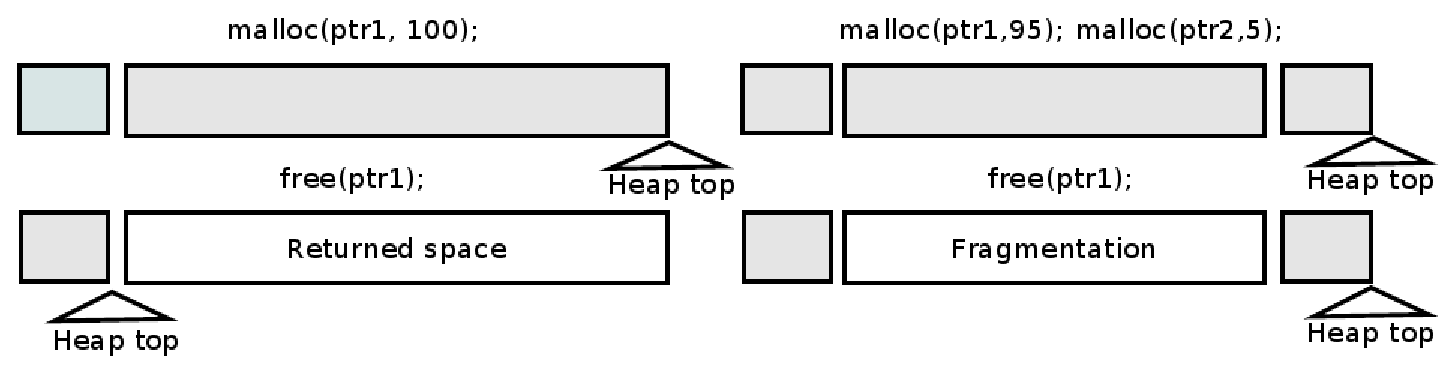
\includegraphics[keepaspectratio,width=1.0\textwidth]{fig/fragmentation}
\end{center}
\caption{Emergence of fragmentation in two scenarios}
\label{fig:fragmentation}
\end{figure}

It can be clearly seen that fragmentation can vary even in different times during
the execution of a single program. This can be a problem especially for a long
running programs doing lot of allocations and deallocations, like daemons or web
browsers. If a bad memory allocator is used, the amount of memory wasted by
fragmentation can rise over time, slowly deteriorating the performance of the
whole operating system. In extreme cases, the allocator can run into problems by
exhausting the whole available memory, while having a large amount of unused
memory \cite{DSAsurvey}. A repeated allocation scenario from the last paragraph
on the heap-based allocator could lead to such situation.

\section{Variables influencing memory allocator performance}
\label{variables}

In previous section, various metrics having a relevance as performance ones were
described. This section discusses factors influencing these metrics. Knowledge of
these factors is needed in order to provide a framework for allocation scenario
creation.

\subsection{Systemcall costs}

When an allocator needs to provide more memory, but it has no suitable free space
available, it has to ask the operating system for more memory. This is done by
appropriate system calls. Linux kernel provides these two system calls suitable
for this purpose.

\begin{enumerate}
\item {\tt brk} system call sets the end of program's data segment to some
certain address. It can be used to enlarge or shrink the segment \cite{posix,
sbrk-manpage}. \item {\tt mmap} system call maps certain amount of memory into
the process address space. This is usually used to map a file to memory, so it
can be read and written via means of normal memory operations, not reads and
writes. But (using the MAP\_ANON flag) it can also be used to allocate anonymous
memory, which is not associated to any specific file \cite{posix, mmap-manpage}.
\end{enumerate}

Additionally, there is a {\tt sbrk} function, provided by C library. This is
basically a wrapper over {\tt brk} system call, providing interface for relative
(as opposed to absolute in the case of {\tt brk}) adjustment of data segment
break \cite{sbrk-manpage}.

System calls are usually considered as expensive operations (due to control
transfer to the kernel and back to userspace), so allocators usually try to map
several allocation requests to single system call and doing internal bookkeeping
on the memory. For this to be effective, the bookkeping must take less time then
it would take so do a simple syscall.

System call cost is a factor affecting the allocation speed. The size of this
influence depends on how often the allocator uses system calls. Allocator doing
one huge memory request once in a while (with bookkeeping on the memory) will
depend on system call much less then one which does a system call for every
allocation request.

\subsection{Size of an allocation}

Size of an allocation can theoretically affect allocation speed, fragmentation
and spatial layout/locality metrics. The impact on speed should, in theory, be
quite minor. It should be slightly easier to find a suitable place for a small
chunk request for a big one (because the allocator can split every large chunk to
several smaller ones, but it can not coallesce smaller, non-adjacent ones), but
the allocator usually knows how large chunks it can provide at the moment, and
for how large more memory should be requested from the operating system.

The impact on memory layout and fragmentation is higher. A larger chunk request
means less possible places to put it into. This is limiting in how "well" the
allocator can place the chunk. The allocator can have a lot of free space
available, but if a request for a chunk just as large as the largest free
continuous space comes, the allocator has only two choices. First choice is to
place the chunk into the free place, possibly worsening locality or memory
layout. The second one is to get more more memory from the operating system to
place the chunk well from the locality point of view, but increasing
fragmentation.

\subsection{Allocation and deallocation order}

The allocation and deallocation order has a major impact on how the fragmentation
metric will look like during the usage of an allocator. As it was described in
subsection \ref{metrics:fragmentation}, some combinations of allocation size and
their ordering can cause "holes" in the memory managed by the allocator.

\subsection{Threading}

Multi-threaded programs are bringing the whole new level of complexity into the
memory allocation system. Threading (and distribution of memory allocations
across threads) can affect all of the performance metrics described in section
\ref{metrics}.

The memory allocator can be considered as a resource for the program. In a
multi-threaded program, any thread can request an allocation or free memory at
any time. If an allocator would not be enabled for multi-threaded environment,
race conditions would probably occur, resulting into several threads using the
identical memory area and rewriting each other's data. To avoid this, the
allocator has to have some kind of control. Such a control could be a locking
scheme, which would serialize the allocation requests of threads. The scheme can
be one large lock, or a finer grained locking scheme, introducing a pipeline.
Another approach is to create an internal thread specific "arenas". Every thread
has it's own "arena" in the allocator, and it's requests are satisfied by using
memory exclusively from it, which eliminates a need for locking. This second
approach is used in the GNU C Library's malloc. Main drawback of this approach is
a higher memory consumption of such an allocator, because every arena has it's
own overhead and fragmentation. This phenomenon is called {\em memory blowup}.

The impact on allocation speed is obvious, and has two sources. Locks in the
allocator cause the threads asking for memory to wait for each other, which could
introduce a major speed reduction of allocation if threads are doing lot of
memory requests. The second source is the overhead of the multi-threading
capabilities of the allocator itself. Both locks and the thread specific "arena"
mechanisms have some overhead, which would be unnecessary in single-threaded
environment.

Second metric where the number of threads has some relevance is the memory layout
and locality. Measuring the false sharing prone allocations only makes sense in
multithreaded environment, because false sharing can only occur when a program
runs simultaneously on at least two CPUs. Locality metric should be measured
inside single thread, and in each thread in multithreaded environment.

\chapter{Benchmarking methodology}
\label{methodology}

In chapter \ref{metrics}, several metrics with some relevance to the performance
of an allocator were analysed and described. This chapter will discuss the
methodology of measuring these metrics.

\section{Measuring memory overhead and fragmentation}
\label{methodology:fragmentation}

The benchmarking tools should be agnostic to the measured memory allocator, in
order to be useful as an universal memory allocator benchmark. This means it
should not depend on any internal knowledge of the allocator, nor it can use some
allocator specific APIs. Using these would mean the benchmark would be unusable
for analysis of the allocators which do not implement these APIs. The benchmark
can only use the standardized {\tt malloc} and {\tt free} interfaces, with
perhaps the future addition of {\tt realloc} interface. In addition to these
APIs, the benchmark can also use some external tools to observe the behavior of
an allocator.

This brings a problem with measuring the memory overhead of an allocator. All the
means benchmark can use only observe the communication of an allocator with the
environment. The benchmark only knows two things. It knows how much memory is
actually allocated by the program. It also knows how much memory the allocator
manages: the benchmark can intercept and log the memory requesting system calls
or it can analyse the memory image of a process to discover the size of the heap.
From these two numbers, the benchmark can compute how much memory is not used in
program, but is granted by the operating system. There is no universal mean how
to discover how much of this unused memory is actually memory overhead (and is
used by the memory allocator metadata) and how much is fragmentation (and is not
used at all). This information is a completely internal in the allocator. Some
memory allocators provide the APIs to determine this information, but it is not
universal, so the benchmark cannot use it.

At least fragmentation is a very important metric, so because the benchmark
cannot reliably measure these two metrics separately, the bechmark has to measure
at least some information which will give some information about the
fragmentation. The approach chosen is to measure just the total amount of memory
which is not used by the program. This value is a sum of fragmentation and memory
overhead. This does not give a precise information about any of these metrics,
but gives an information about how effectively the allocator manages it's memory.
After all, from the outside, these two metrics share the most important
characteristic: they both represent an amount of memory granted by the operating
system, but it cannot be used in the program. This new {\em unused memory}
metric's absolute value can be taken after each allocation and deallocation. From
these values, a unused memory ratio can be calculated and statistically
processed.

In addition to this, a real fragmentation metric can be calculated by detailed
analysis of allocation and deallocation requests, and detecting if such request
caused a system call. If an allocation request was done and satisfied without an
system call being issued, it is certain that at the time of an allocation request
the memory was free and unused in the allocator's managed area, and therefore
considered as fragmentation. If another allocation request is made and no system
call is still caused by it, we can add this value to the previous one: at the
time of the previous allocation request at least the space of the sum of these
two allocations were fragmented for sure. When a system call for more memory is
issued, the knowledge about fragmenation is invalidated and the computation has
to start again. A system call returning memory to the operating system does not
invalidate this value. Similar thing can be observed for deallocation requests.
If a deallocation request does not cause an allocator to return the memory to the
operating system, it is kept in the allocator and considered as fragmentation.
Subsequent cases can be summarized too, and invalidated by the system call
returning memory. This gives a limited information about fragmentation - it is a
minimal amount of fragmentation in that precise time. Usefulness of this metric
is limited to the concrete usage scenarios and allocator characteristics: for
most of the scenarios mixing allocation and dealocation requests these values
will be invalidated often, limiting their precision.

\section{Measuring allocation speed}

Measuring the speed of a single allocation is not relevant enough. In a
multitasking environment, there are many side factors which can affect the
allocation speed. The time of a single allocation is also very small, meaning any
side effect will affect the measurement by a large mean and bring considerable
error to the measurement. To obtain at least some precision, the measurement
method should be statistically sound. This means a sufficiently large set of the
identical experiments has to be done. The results of this set should be processed
statistically. Second issue to be considered is the differentiation of time spend
in userspace (which means in the allocator itself) and in the kernel, doing work
in the system calls. These two time metrics should be taken separately. While the
time spent in an allocator is a interesting metric by itself, the system call
costs are not. System call costs are considered as an input in the system: they
can change and the allocator has no control on how long the system call will
take. The tool has to allow the user to specify also the system call costs in the
environment, to find out the predicted allocator performance in such an
allocator. This cost should be implemented as a function of the allocation size,
with the possibility to incorporate some amount of pseudo randomness into this
function. At least the means to specify standard and uniform distribution should
be provided. With these abilities, it should be possible to describe the most
important characteristics of the system call cost: dependence on the system call
allocation size, constantness and some random changes in behavior of the kernel.

The exact method of measuring duration of a single allocation request should be
saving the time (or the contents of the clock counting registers) first before
the allocation, second after the allocation. The difference between these two
numbers yields the total time spent in allocation, including the time spent in
the kernel. The time spent in the kernel should be traced via an external tool.
There are also some external effects present, so the resulting time will not be
precise enough, but it could be useful e.g. in comparison done in the same
environment.

There is another problem in measuring time. There are also context-switches,
which can prolong the measured times. In some cases, these durations are
interesting: time spent waiting in the kernel is interesing in the case of
multiple threads doing allocations using an allocator with locks. Locking will
slow down the execution of the program. This effect is interesting enough to
measure. For this purpose, the tool should provide the ability to measure the
execution not by per-allocation basis, but also on total program execution basis.
This will incorporate also the effect of lock contention by threads. Doing
statistical analysis of the sufficient number of experiments, the effects of any
accidental interference (context switches to another programs and similar) should
be mitigated in the resulting value.

\section{Measuring locality and memory layout}
\label{methodology:locality}

Analysis of the memory layout should not be very hard. The tool has complete
information about the positions of the allocated memory as well as the size of
it. Using this information, it can construct an image of how the memory looks
like. From this image, it's easy to see how far from each other the allocated
memory chunks are. There is also a drawback: because of virtual memory mechanism
in place, the benchmark cannot reliably tell if chunks close to each other in the
process' address space are close even in physical memory. The process' continuous
memory space can be assembled from several fragmented physical memory pages. So
the proximity in process space does not imply the proximity in physical memory,
and by extension, the real locality. But the locality would be broken only on the
boundaries of the physical memory pages. Most of the allocated data should be
inside the pages, which means the better proximity in process space means higher
probability of having better real locality.

Inside single thread, the measured metric should be the locality of two allocated
chunks of memory based on the temporal proximity. The absolute distance between
two chunks of memory can be computed as a difference between the end of the chunk
with higher address and the address of the chunk with lower address. The absolute
distance depends on the sizes of these two chunks, so for the purpose of having
the metrics comprarable we will relativize it:
\begin{displaymath}
DISTANCE_{rel} = \frac{size_1 + size_2 + gap}{size_1 + size_2}
\end{displaymath}
The numerator of the fraction is the absolute distance, and by dividing it by the
sum of sizes, we obtain a relative locality metric. A value of 1 means there is
no gap between the two chunks, meaning the best locality. The higher number means
worse locality. This metric will be taken for each pair of a specific temporally
distant allocation. This will allow to compute the average locality of each
temporal distance - temporal distance 1 means the allocation requests were issued
one just after the other, distance 2 means the two allocations had one more
between them, and so on.q

Across multiple threads, a similar metric should be taken for determining of the
possibility of false sharing. The closer the two memory chunks allocated in
different threads, the higher is the probability of false sharing if these two
chunks were used simultanneously in their owner threads. For each two threads in
the system, the tool will find the sizes of gaps between the chunks belonging to
different threads. From the detailed analysis of sizes of these gaps it will be
possible to find out the minimal gap size to determine of any false sharing can
occur at all for the given cache line size, as well as the number of memory
chunks which could cause false sharing if used simmultaneously.

Another approach to analyse locality in a rather practical way is to do some
computing on the allocated memory, and observing cache misses on various levels
occuring during the runtime. In multithreaded environment, the misses count will
probably heavily depend on the execution order of the threads, which means more
experiments will have to be done for obtaining numbers with higher precision.

\chapter{OSMB toolset}

This chapter will discuss the design and implementation of the tool. OSMB is a
abbreviation of "Open Source Malloc Benchmark".

\section{Design}

The toolset will be composed from several smaller tools which will measure
various metrics as described in previous chapter. This approach was chosen
because of the better precision of the measurement. If all the metrics were taken
during one benchmark run, some metrics, especially the time ones, could be
affected by the overhead introduced by the benchmark. At least for the time
performance metrics the benchmark tools should have as low overhead as possible.
In contrast to this, for fragmentation and memory layout analysis there is no
need for this, because the goal is to obtain precise results even for the price
of some duration overhead.

To allow the user to specify the environment for testing, i.e. the values of the
various factors as described in \ref{variables}, the tool will take a {\em
scenario file} as an input. This file will be written in a domain specific
language, and will specifify how all of these variables, or a subset of them will
look like in the environment. This file will serve as input to the {\em scenario
driver}, which will parse it and will execute one run of such a scenario. During
the execution, one or more measurement tools will attach to the driver, and will
take the metrics. The tool should allow the user to run the scenario for the
specified number of times, obtaining results from all of these runs, and then
perform some statistical analysis of the collected data. To mitigate the effect
of "warming up", the tool should provide the ability to run the arbitrary number
of unmeasured executions.

There are two sources of the scenario input files. The format will be text based
domain specific language, so the user can manually write the scenarios, or write
a generator. One such generator should be provided with the tool. The generator
should be able to attach to any running process which uses dynamic memory
allocation, and trace it's usage of {\tt malloc} and {\tt free}, creating a
scenario file from the collected information. Tracing these functions will be
done by using external tools: ltrace or Systemtap.

The measurement tools should not do any unnecessary computing during the
benchmark execution. They should only record the observations. These raw data
should be processed after the benchmark execution. The toolset should also
provide some tools for processing, interpreting and visualization of these raw
data.

The measurement tools' function will we be direct implementation of the
principles in chapter \ref{methodology}. The design for the remaining parts of
the suite is described in the following subsections.

\subsection{Scenario driver}

The scenario driver will be the central piece of the whole suite. It will take
the scenario file as an input, parse it and create a program image of the
scenario by the instructions in the input file. It will then hook the specific
measurement tools into this generated program. The result will be compiled using
standard C compiler. The resulting binary program is the representation of one
run of the described scenario. This scenario will be run multiple times, and
during its execution the external observation tools will attach to it. The output
of these external tools, combined with the output of the scenario binary itself
is the result of the benchmark.

\subsection{Tool for system call catching}

Some of the metric measurement tools will benefit from the system call
observations. There are two kinds of system calls which can occur during the
benchmark execution. First are the memory allocation related system calls. These
should be recorded with the parameters showing how much memory was processed by
them. The rest are the system calls unrelated to memory management. These will be
not recorded at all. If it would be possible to record only the system calls
coming from the allocator itself, and not e.g. the measurement tools, maybe it
would be useful to track some others, like the locking related ones, like {\tt
futex()}. This is easily achievable with existing tools, like strace, so the
focus of this work won't be on this use case.

\subsection{Scenario recorder}

The recorder will attach to any running program and trace it's usage of memory
allocation functions. Tools like ltrace \cite{tools:ltrace} or systemtap
\cite{tools:systemtap} will be used for this. The data collected from this trace
will be translated into the scenario file, and then can be used independently on
the original program. Analysis of such a scenario can be used to tell if some
non-standard memory allocator would improve the performance of the original
program. The recorder will have to be able to distinguish the memory allocations
requests done by multiple threads, in order to correctly replicate the memory
allocation scheme of the recorded program.

\section{Data analysis tools and desired output}

The output of the benchmark run will have the form of the raw data, with no
particular information in them. The suite will also provide several tools to help
the user analyse and interpret these raw data. The tools should provide tools for
finding at least these outputs:

\begin{itemize}
\item Unused memory ratio. The maximal, minimal, average, median, mean, quartil
values and standard deviation should be reported. Also, the graph showing the
unused memory ratio per run should be provided. Additionally, a third graph
should be reported, showing the progression of the unused memory ratio dependent
on the allocation and deallocation request during the time of an execution.
\item Duration of one run. The maximal, minimal, average, median, mean, quartil
values and standard deviation should be reported. The graph showing the duration
per run should be provided. The purpose of this graph is to quickly recognize and
compare the speed stability of the allocators. Such an instable allocator would
have large standard deviation compared to the average values, and this can be
easily seen in a graph. Additionally, a graph showing the predicted speed of one
run dependent on the system call cost should be provided, with the actual average
system call cost highlighted. \item Duration of one allocation. Per each run, the
tool should report minimal, maximal, average, mean, median, quartils and a
standard deviation of a allocation duration. This metric can be taken in time or
in CPU cycles. A graph showing the duration of allocations during one run should
be reported. \item Fragmentation. The fragmentation metric found out as described
in section \ref{methodology:fragmentation} should be reported just per one run.
Because the number of measured values need not necesarilly stay the same in more
executions of the scenario, the values are not easily comparable. Per one run, a
minimal, maximal, average, median, mean and quartil values should be reported.
The standard deviation should be also reported. In addition to this, the graph
showing the progression of fragmentation during one execution of the scenario
should be provided. Because the value of fragmentation can be unknown for some
allocation and deallocation requests, the graph should highlight these
allocations as unknown value to avoid confusion of misunderstanding of the graph.
\item Locality and memory layout. For each thread in the system, a maximal,
minimal, average, mean, median, quartil values and standard deviation should be
reported for these metrics: absolute value for the "gap" between two blocks and
relative locality metric as described in \ref{methodology:locality}. This output
is supposed to be computed for any temporal distance of allocations in the
system. Also, for the input sizes of a cache line and each run, the system should
report a percentage of temporally close allocations which could theoretically fit
into that cache line of that size but are placed in a way prohibiting this,
representing a missed optimalization opportunity. Last memory layout metric to be
reported is the minimum, maximum, average, median, quartils and standard
deviation of the absolute distance between two blocks owned by different threads.
Analogically, a percentage of block pairs which could cause false sharing for an
input size of a cache line should be reported. \item Memory layout visualization.
For each allocation during one run of a scenario, a visual image of process'
address space should be reported for easy visualization of the allocator's
function.
\end{itemize}

All of the graph outputs would provide the ability of showing the results of the
several runs in one graph, providing easy comparison of them.

\section{Implementation}
\subsection{Scenario infrastructure}
The tool is based on the idea of measuring the allocator performance on any
memory allocation scheme. The tool has to be able to create a correct working
program which will allocate and deallocate memory based on this scheme. To
describe schemes, the infrastructure around {\em scenarios} was created.
{\em Scenario} is a description of a memory allocation scheme, described in a
domain specific language. This description is then translated to a valid C
program, which is then compiled using standard C compiler. The resulting binary
is an isolated testcase usable for various performance metrics measurement. 
\subsubsection{Scenario files}
For the purpose of describing memory allocation scheme, a simple language was
created. Later in this text, it will be called {\em scenario language}. The
language is text-based, and it was created to allow simple readability by a
human. This means several needless keywords were added just for the purpose of
the statements forming a sentence similar to natural English language.

The scenario language allows to describe all aspects of programs using memory:
threaded environment, allocations, deallocations and working with allocated
memory. Allocations, deallocations and work are represented by a {\em command}
statements. For allocations, command specifies the amount of memory (in bytes)
to allocate, and an identifier of an variable pointing to the memory.
Deallocation command specifies the variable identifier which will be passed to
{\tt free} call. Work command is a bit more complicated. To allow a flexible
control of the work being done with allocated memory, the user can specify four
arguments to work statements: type, amount, identifier and direction. There are
four {\em types} of work which can be done with memory: reading, writing and the
two combinations of these: read followed by immediate write and vice versa. The
{\em amount} of work specifies the number of bytes with which the work will be
done. It can be specified as {\em whole} or {\em random}, which means a random
sample of possible indexes (of random size) will be selected for work. {\em
Identifier} is the variable holding memory with which the work will be done.
{\em Direction} specifies the order in which the indexes will be used; there can
be three values: sequential, backwards and random.
All choices described here as random are made when the scenario file is
translated to the C program. The generated C program is then fully
deterministic.

{\em Commands} are grouped to named {\em workjobs}. Workjob is a sequence of
commands, and represents one basic block of C code. {\em Threads} can be
specified with their numeric identifier, the workjob they will perform, and the
number of iterations the thread will perform of that workjob.

In addition to the specification of threads and workjobs, the scenario describes
limits to the execution: the user can specify the memory limit in bytes, and the
maximum number of threads.

The example of scenario file is in figure \ref{scenario-sample}. The example
shows a single workjob called {\tt w1} consisting of an allocation of 5-bytes
array, doing some artifical work on this array, and deallocating it. Three
threads are are all performing this identical workjob, but the number of
iterations is different. First thread will perform 100 iterations of {\tt w1},
second one 500 and third one 1000 iterations. Thread limit is set to three, so
the translator would not allow an addition of another thread. Memory limit is
set to 1024 bytes, which is totally sufficient for this case (every thread can
have 5 bytes allocated at most, and there are three threads: no more then
15 bytes will be allocated at any time). If the allocation size in workjob would
be changed to 500, then the translator would end with error: three simultaneous
threads could allocate 1500 bytes of memory, which is higher than the limit.  

\begin{table}[h]
\begin{center}
\begin{lstlisting}[frame=single]
memory-limit = 1024
threads      = 3

workjob w1 = {
  alloc one 5

  work read whole one sequential
  work write whole two sequential
  work rw random three random
  work wr random three backwards

  dealloc one
}

thread 1 does workjob w1 times 100
thread 2 does workjob w1 times 500
thread 3 does workjob w1 times 1000
\end{lstlisting}
\caption{Example scenario file}
\label{scenario-sample}
\end{center}
\end{table} 

\subsubsection{Scenario translator}
The scenario translator is written in Python and consists of three simple parts:
parsing, validating and generating. The parsing part is written using PLY
complier construction tools~\cite{python-ply}. The output of the parser is the
{\tt Scenario} instance. 

Several validations are done on the parsed scenario. The scenario semantics is
analysed by browsing through commands in all workjobs. Using this information,
two types of invalid actions are identified: {\em work} and {\em dealloc} 
commands on a variable which does not have any memory allocated at the moment.
These are clearly invalid actions: if these commands were allowed, the resulting
C program would contain code either working in or freeing the unallocated
memory. Memory allocation to a pointer already pointing to allocated memory is
not considered an invalid action by default. The resulting program will contain
memory leaks, but this does not make the program invalid: the behavior of such
program is still defined. This decision was made based on the requirement of
scenario creation based on traces of real programs allocation scheme: this
program will most probably contain some leaks too. In the case of memory
leak-free testcase need, the safeguard prohibiting leaks can be switched on by a
configuration option.

The second type of a validation performed by a translator is the conformance
with the set limits. The check for number of threads is straightforward. For the
memory consumption limit, the analysis allows a computation of maximum memory
consumption of a thread. The sum of maximum values is checked to be lower
then this limit.

C program is then generated from a scenario found to be valid. For each thread,
one function is generated. This function contains one {\tt for} cycle. The body
of this cycle will be performed {\em n}-times, where {\em n} is the number of
iterations set in the thread definition. The body of the cycle consists of a
block generated from an appropriate workjob definition. The workjob is
translated as a sequence of statements.

The allocation command is translated to an assignment of {\tt malloc} return
value to the pointer with appropriate identifier. First allocation to pointer is
translated to a assignment declaration instead. Both variants are shown in table
\ref{scen-translate-table}. The deallocation is simply translated as a free
statement of an appropriate pointer.

The work statements are more complicated. There are 24 variants of what can be
generated from various forms of this statement. Straightforward variants
(reading and/or writing the whole array either sequentially or backwards) are
translated as {\tt for} cycles looping the appropriate commands. In the case of
random order or random part of the array, the command is translated to the
sequence of appropriate statements. The statements are shown in table
\ref{scen-translate-table}. To illustrate the whole translation, the example
scenario from figure \ref{scenario-sample} is shown translated to C in figure
\ref{scenario-sample-trans}.

\begin{table}
\begin{center}
\begin{tabular}{|l|l|}
\hline
Scenario language & C language \\ \hline \hline
alloc one 256 (first occurence) & {\tt char *one = malloc(256);} \\ \hline
alloc one 256 (next occurences) & {\tt one = malloc(256);} \\ \hline
dealloc one & {\tt free(one);} \\ \hline
work read \ldots one \ldots & {\tt helper = one[iterator];} \\ \hline
work write \ldots one \ldots & {\tt one[iterator] = random\_value;} \\ \hline
work rw \ldots one \ldots & {\tt helper = one[iterator];} \\
& {\tt one[iterator]= random\_value;} \\ \hline
work wr \ldots one \ldots & {\tt one[iterator]= random\_value;} \\
& {\tt helper = one[iterator];} \\ \hline
work \ldots sequential & {\tt for(long i=0; i<size; i++)\{\ldots\}} \\ \hline
work \ldots backwards & {\tt for(signed long i=size-1; i>=0; i--)\{\ldots\}} \\
\hline
\end{tabular}
\caption{Command translations}
\label{scen-translate-table}
\end{center}
\end{table}
\begin{table}
\begin{center}
\begin{lstlisting}[frame=single, basicstyle=\tt\footnotesize, language=C]
// Malloc benchmark file generated on 2010-04-04
// Limits:
//   Memory limit: 1024
//   Threads:      2
#include <stdlib.h>
#include <pthread.h>

void *function_1_w1 (void *arg){
	char helper;
	for (long iteration = 0; iteration < 100; iteration++){
		char *one = malloc(5);
		for (long iterator=0; iterator < 5; iterator++){
			helper = one[iterator];
		}
		one[1] = 33;
		one[4] = 33;
		one[2] = 33;
		for (signed long iterator=4; iterator >= 0; iterator--){
			one[iterator] = 96;
			helper = one[iterator];
		}
		free(one);
	}
}

void *function_2_w1 (void *arg){
	char helper;
	for (long iteration = 0; iteration < 500; iteration++){
		char *one = malloc(5);
		for (long iterator=0; iterator < 5; iterator++){
			helper = one[iterator];
		}
		one[3] = 125;
		one[4] = 125;
		for (signed long iterator=4; iterator >= 0; iterator--){
			one[iterator] = 12;
			helper = one[iterator];
		}
		free(one);
	}
}

int main()
{
	pthread_t thread1;
	pthread_t thread2;
	pthread_create(&thread1, NULL, function_1_w1, NULL);
	pthread_create(&thread2, NULL, function_2_w1, NULL);
	pthread_join(thread1, NULL);
	pthread_join(thread2, NULL);
	return 0;
}
\end{lstlisting}
\caption{Example translation}
\label{scenario-sample-trans}
\end{center} 
\end{table}
 
\subsubsection{Scenario capture}
Two approaches were chosen for the tool allowing to capture a memory allocation
scheme of a program: Systemtap tracing script\cite{systemtap} and a library
containing wrappers for {\tt malloc} and {\tt free} functions. Both approaches
were implemented, because they have different limits and advantages. The capture
itself consists of two stages: tracing and analysis. At runtime, simple trace of
memory allocation calls is created. To avoid performance hits on the traced
program, no analysis is being performed on the trace at runtime. Every memory
allocation request is recorded with the following information: TID, PID,
requested size and the memory address of the chunk the allocator returned. This
is needed to identify which chunks are being freed by the program: this address
is the argument of the deallocation call. Deallocation requests are recorded with
PID, TID and the address being freed. The full trace is then analysed and
translated to the scenario file.

Systemtap tracing is very straightforward. Systemtap allows to hook probes to
return from function event. It also provides access to function arguments, return
value and several helper functions returning information about the environment
where the function is executed: PID and TID of the process. Two probes exist: one
for {\tt malloc} and second for {\tt free} calls. These probes just print the
appropriate data whenever any thread goes through the return from {\tt malloc} or
{\tt free}. The advantage is simple and reliable use. The disadvantage is that
the user has to know the location of the actual function code (which
binary--library or executable--contains this code). The user needs DWARF
debugging information for this binary. However, in most cases, this location will
be the system C library (usually GNU C library) and most distribution provide
separate DWARF debugging information in separate packages. The second
disadvantage is the need of root privileges to be able to use Systemtap.

Separate library wrapper is usable when the program uses dynamically linked
memory allocator. A LD\_PRELOAD capability of a dynamic loader allows an
additional library to be loaded before all others. Symbols in this library
effectively override those in other shared libraries. Wrappers in this library
need to call the real functions in system library, which is possible by dynamic
lookup of that symbol using the RTLD\_NEXT pseudo-handle~\cite{RTLD_NEXT}.

% \section{Implementation decisions} The implementation itself is beyond the
% scope of this term project, and will be done in future work on the diploma
% thesis. However, several design related decision about implemetation were done
% already.

% The implementation language will be C for the parts directly involved in the
% scenario execution and Python for the scenario file translator and data
% analysis tools. Some tools will be implemented as Systemtap dynamic tracing
% probe scripts. The memory allocators will be linked to the scenario binary
% either directly during the scenario compilation, or using LD\_PRELOAD for some
% specific cases when several allocator will be tested, avoiding the need for
% re-linking the scenario binary for each allocator.

% \chapter{Conclusion}

% This term project had three main goals. This chapter describes the achieved
% work on these goals, and makes conclusions based on these goals.

% \section{Achieved work}

% The inital goal of the term project was to describe the dynamic allocation
% problematics, and identify the features and characteristics important to the
% topic of the thesis. These were described in chapter \ref{dsa}. Several
% performance metrics were identified and described. The identified performance
% metrics were memory overhead, memory fragmentation, allocation speed and memory
% locality and layout metrics. For these metrics, a benchmarking methodology was
% created. The second part of the initial goal was to find the factors affecting
% these performance metrics. These factors were described in \ref{variables}. The
% factors are these: system call cost, allocation request size, the order in
% which the requests are coming, and the number of threads in the application
% using the allocator.

% Using the identified factors and performance metrics, the high-level design of
% the benchmarking tool was designed. The design was driven by the two main
% goals: it has to provide the ability to influence all of the performance
% factors in the benchmarking environment, and it has to be able to measure all
% the performance metrics as presisely as possible, using statistical means where
% necessary. The design also identified the precise output values for each
% metric.

% The whole tool was designed to be a interpreter of a domain specific language,
% encoding the usage scenario of the allocator: both the environmental
% characteristics (system call costs) and the program characteristics (threading,
% allocation size and order). The interpreter will create a C program. The
% execution of this program will then be analysed by the various metric specific
% tools, both during the execution (data collection) and after it (data analysis
% and interpretation).

%\section{Future work}

% Using the factors and metrics collected in this term project, as well as the
% initial high-level design decision, the benchmarking tool suite will be
% implemented. Aside from the implementation itself, the tool will use several
% external tools to do some specific tasks. It will use GCC to compile the
% programs. Systemtap will be used for the userspace-kernelspace communication
% interception, and if possible also to catch the malloc/free calls in the
% userspace. If this is not possible, ltrace will be used.

% When the implementation is ready and working, the tool will be tested on
% several allocators. The main popular ones will be tested, and some interesting
% experimental one too. These candidates for the testing will have to be found.
% \chapter{Different malloc implementations analysis} \chapter{Conclusion} I will
% be Ing. \cite{Pravidla}
% =========================================================================
